\chapter*{Conclusiones y recomendaciones}
\addcontentsline{toc}{chapter}{Conclusiones y recomendaciones}
\markboth{Conclusiones y recomendaciones}{Conclusiones y recomendaciones}

% Las figuras y tablas de este capitulo sin numero se rotulan «CR.1», «CR.2»...
% (no «C», que es el Anexo C). El grupo deshace las redefiniciones al cerrar; el
% primer \chapter de los Anexos vuelve a poner los contadores en cero. \theH...
% da a hyperref destinos propios, distintos de los del Capitulo 3.
% final4 (tribunal, defensa de borrador): conclusiones breves, sin los rotulos
% «Conclusion N» ni «Recomendacion N» y sin las secciones «Aportes del trabajo» y
% «Limitaciones». Lo unico que decian paso a la seccion de limitaciones observadas
% del Cap. 3 (sec:limitaciones-observadas) y a los parrafos de los Cap. 2 y 3 de abajo.
% Cada conclusion abre con su capitulo y con «se concluye que» (decision del autor).
\begingroup
% Las Figuras CR.1 y CR.2 ocupan entre la mitad y dos tercios de la hoja: con los
% valores por defecto, LaTeX las mandaba cada una a una hoja de flotantes, con el
% resto en blanco. Aqui pueden ir arriba de la hoja con texto debajo.
\renewcommand{\floatpagefraction}{0.85}
\renewcommand{\topfraction}{0.85}
\renewcommand{\textfraction}{0.10}
\setcounter{figure}{0}
\setcounter{table}{0}
\renewcommand{\thefigure}{CR.\arabic{figure}}
\renewcommand{\thetable}{CR.\arabic{table}}
\renewcommand{\theHfigure}{CR.\arabic{figure}}
\renewcommand{\theHtable}{CR.\arabic{table}}

\section*{Conclusiones}
\phantomsection\addcontentsline{toc}{section}{Conclusiones}

El trabajo cumplió su objetivo general: desarrolló EduFEM, un software educativo de elementos finitos, libre, en español y escrito en Python, que expone su procedimiento de cálculo en elasticidad plana con elementos Q4 y Q9. La respuesta al problema es que la escasa transparencia del software de análisis oculta las magnitudes intermedias, y sin ellas un resultado no puede seguirse hasta sus datos ni comprobarse paso a paso.

La hipótesis queda comprobada (\autoref{fig:contraste-hipotesis}): sus tres premisas se respaldan, y la trazabilidad y la verificabilidad cumplen todos sus criterios de aceptación. El alcance es el declarado: se midieron propiedades del software, no su uso por estudiantes.

\begin{figure}[!htbp]
\centering
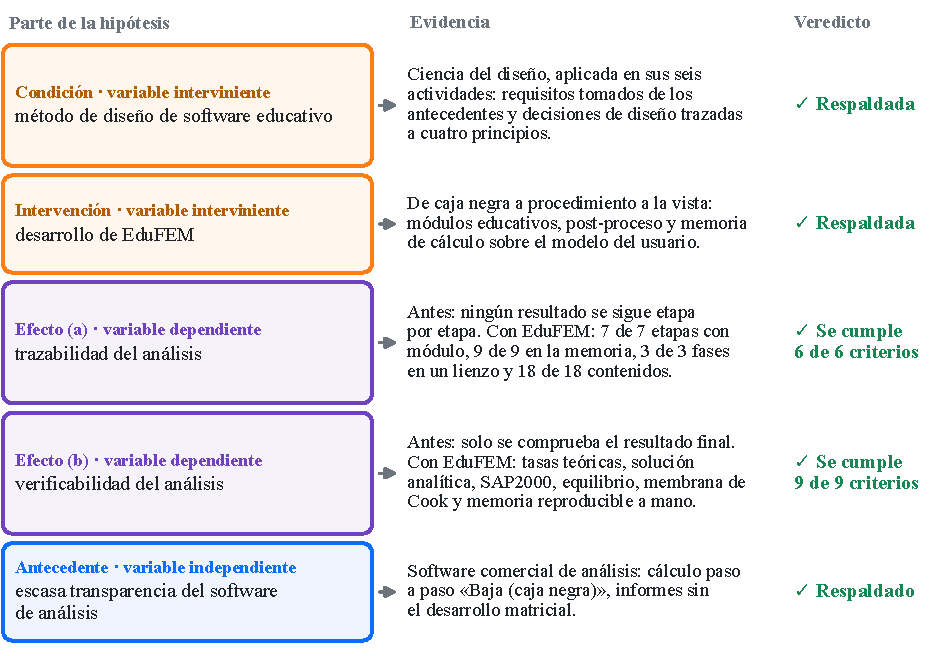
\includegraphics[width=\linewidth]{fig_contraste_hipotesis.pdf}
\caption[La hipótesis, parte por parte.]{La hipótesis, parte por parte: el papel de cada una, su evidencia y su veredicto. El enunciado está en la Introducción (\emph{Hipótesis}) y en la \autoref{sec:validacion-hipotesis}; las cifras proceden de la \autoref{tab:veredicto}, la situación de partida de la \autoref{tab:comparativa} y los veredictos de la \autoref{tab:componentes-hipotesis}.}
\label{fig:contraste-hipotesis}
\end{figure}

De la fundamentación teórica (\autoref{cap:marco_teorico}) se concluye que el software comercial de análisis opera como una caja negra y que ningún recurso educativo revisado documenta a la vez los atributos que harían trazable y verificable el procedimiento de cálculo (\autoref{tab:comparativa}). De esa brecha salieron los requisitos de la herramienta (\autoref{sec:requisitos}).

Del desarrollo de EduFEM (\autoref{cap:diseno}) se concluye que el software lleva su procedimiento de cálculo a la vista: los módulos educativos exponen sobre el modelo del usuario las etapas hasta el ensamblaje, el post-proceso muestra la respuesta con sus medios de comprobación y la memoria de cálculo reconstruye todo el procedimiento con sustitución numérica (\autoref{tab:fases}; \autoref{fig:fases-lienzo}). Las decisiones de diseño que lo logran, trazadas a sus principios (\autoref{tab:principios}), son un aporte reutilizable del trabajo.

De la verificación y la validación (\autoref{cap:resultados}) se concluye que ese procedimiento es trazable y verificable (\autoref{tab:veredicto}), que los criterios numéricos se cumplen con amplio margen (\autoref{fig:margen-criterios}) y que quedan respondidas las dos preguntas de investigación. La batería que establece la verificabilidad, reproducible y publicada con el software, es otro aporte del trabajo.

\begin{figure}[!htbp]
\centering
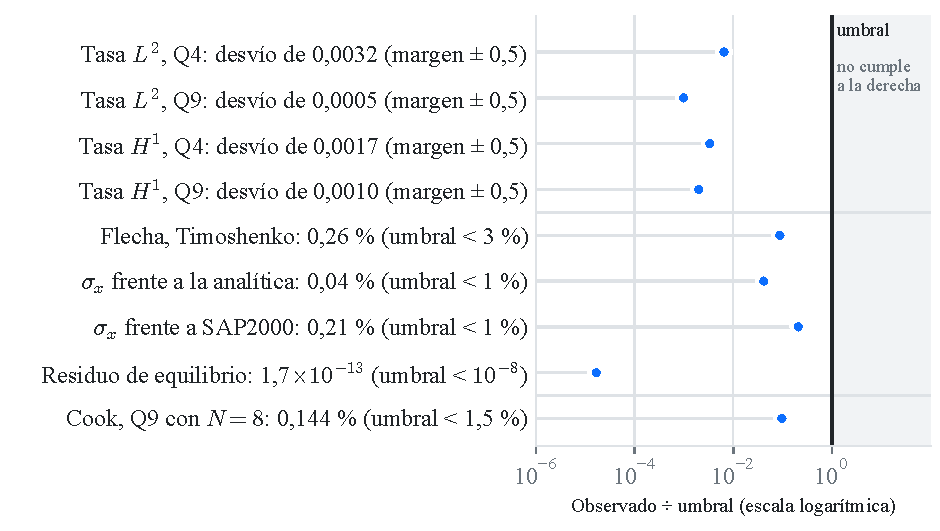
\includegraphics[width=\linewidth]{fig_margen_criterios.pdf}
\caption[Margen de cada criterio numérico de la cláusula (b).]{Margen de cada criterio numérico de la cláusula (b): el valor observado dividido por su umbral, en escala logarítmica. Todos los puntos quedan a la izquierda del umbral; cuanto más a la izquierda, más lejos del incumplimiento. En las tasas de convergencia se grafica el desvío respecto de la tasa teórica, en la peor de las cuatro configuraciones ensayadas. Las cifras son las de la \autoref{tab:veredicto}, salvo los desvíos, calculados con las tasas sin redondear.}
\label{fig:margen-criterios}
\end{figure}

El desarrollo tuvo un inconveniente: la lectura de la memoria de cálculo delató un defecto en la extrapolación de tensiones del Q4 que las pruebas de convergencia no mostraban. Se corrigió, y una prueba de la batería lo detectaría hoy (\autoref{sec:leccion-extrapolacion}); el episodio muestra, además, que exponer el procedimiento no asegura que lo expuesto sea correcto. Quedan tres debilidades, que detalla la \autoref{sec:limitaciones-observadas}: la evaluación es del autor, la deformación plana no tiene contraste externo y la exposición del procedimiento es una posibilidad que el software ofrece, no un recorrido que imponga.

% La Figura CR.2 respalda la conclusion del Cap. 3: la barrera impide que caiga
% bajo el titulo «Recomendaciones» y parta en dos la primera de ellas.
\FloatBarrier
\section*{Recomendaciones}
\phantomsection\addcontentsline{toc}{section}{Recomendaciones}

Las recomendaciones nacen de las debilidades señaladas y de las fronteras del alcance (\emph{Alcance y limitaciones}). Se agrupan por capítulo, y la \autoref{tab:triada} reúne la tríada completa.

% \needspace: el titulo de cada grupo no queda solo al pie de una hoja, separado de su
% primera recomendacion (le paso al del Cap. 3 al recortar las Conclusiones).
\needspace{4\baselineskip}
\noindent\textbf{Para la fundamentación teórica (\autoref{cap:marco_teorico}).}
\begin{itemize}
    \item \textbf{Tratamiento del bloqueo.} Incorporar la integración reducida selectiva o la formulación $\bar{\bm{B}}$ \autocites[pp.~221, 232-234]{hughes2000fem}[pp.~476-477]{bathe2014fem}, con un módulo que contraste, sobre un mismo modelo, la respuesta bloqueada y la corregida (\autoref{sec:locking}).
    \item \textbf{Más tipos de elemento.} Agregar triángulos lineales y cuadráticos, y cuadriláteros de ocho nodos y de transición \autocites[pp.~167-174, 194]{onate2009structural}{reddy2006introduction}.
\end{itemize}

\needspace{4\baselineskip}
\noindent\textbf{Para el desarrollo del software (\autoref{cap:diseno}).}
\begin{itemize}
    \item \textbf{Mallado automático.} Un generador sobre el contorno dibujado en el lienzo, controlado por las métricas de calidad del módulo M0.
    \item \textbf{Solucionador para mallas muy grandes.} Una factorización de Cholesky y un solucionador iterativo precondicionado (\autoref{tab:tiempos}), sin perder la versión legible del ensamblaje.
    \item \textbf{Guía docente.} Una secuencia de prácticas que acompañe al manual del \autoref{anexo:manual}, como rehacer a mano una etapa de la memoria del ejemplo guía.
    \item \textbf{Extensión a tres dimensiones.} Hexaedros y tetraedros, que se formulan con la misma base isoparamétrica.
\end{itemize}

\needspace{4\baselineskip}
\noindent\textbf{Para la verificación y la validación (\autoref{cap:resultados}).}
\begin{itemize}
    \item \textbf{Ampliación de la batería.} Agregar un caso civil en deformación plana con solución publicada, un caso con carga superficial linealmente variable y una prueba propia del término de cortante de la matriz de deformación plana, y medir el error de tensiones del Q4 sin la franja de contorno (\autoref{sec:mms}).
    \item \textbf{Revisión independiente.} Someter la tabla de cobertura al juicio de docentes o de especialistas en el MEF, y el código del motor a una revisión por terceros. El uso de la herramienta en el aula queda para una investigación educativa distinta.
\end{itemize}

\begin{table}[H]
\centering
\caption[La tríada: capítulo, conclusión y recomendaciones.]{La tríada del trabajo. Cada fila se lee de izquierda a derecha: el capítulo y el objetivo específico que cumple, la conclusión que establece con la evidencia que la respalda, y las recomendaciones que deja.}
\label{tab:triada}
{\footnotesize
\setlength{\tabcolsep}{3pt}
\renewcommand{\arraystretch}{1.25}
\begin{tabular}{@{}>{\raggedright\arraybackslash}p{2.7cm}@{\hspace{4pt}$\rightarrow$\hspace{4pt}}>{\raggedright\arraybackslash}p{6.3cm}@{\hspace{4pt}$\rightarrow$\hspace{4pt}}>{\raggedright\arraybackslash}p{5.2cm}@{}}
\toprule
\textbf{Capítulo y objetivo} & \textbf{Conclusión y evidencia} & \textbf{Recomendaciones} \\
\midrule
\autoref{cap:marco_teorico}. Fundamentar (cumplido) & Ningún recurso revisado documenta a la vez los atributos que harían trazable y verificable el procedimiento; de esa brecha salen los requisitos (\autoref{tab:comparativa}; \autoref{sec:requisitos}) & Tratar el bloqueo (integración reducida selectiva, $\bar{\bm{B}}$) y ampliar la biblioteca de elementos \\
\autoref{cap:diseno}. Desarrollar (cumplido) & EduFEM expone el procedimiento a la vista sobre el modelo del usuario: módulos y post-proceso sobre un mismo lienzo, y memoria de cálculo (\autoref{tab:fases}; \autoref{fig:fases-lienzo}) & Mallado automático, solucionador para mallas muy grandes, guía docente y extensión a tres dimensiones \\
\autoref{cap:resultados}. Verificar y validar (cumplido) & El procedimiento es trazable y verificable: se cumplen todos los criterios de aceptación (\autoref{tab:veredicto}; \autoref{fig:contraste-hipotesis}; \autoref{fig:margen-criterios}) & Ampliar la batería (deformación plana, carga variable) y someter la tabla de cobertura y el código a revisión independiente \\
\bottomrule
\end{tabular}}
\end{table}

\endgroup
